\chapter{Analiza struktury zastosowanego oprogramowania}
\section{Połączenie z czujnikiem temperatury MLX90614}

Czujnik temperatury MLX90614 został podłączony do mikrokontrolera Arduino za pomocą interfejsu I2C. W celu komunikacji z czujnikiem została wykorzystana biblioteka Wire.h. W celu sprawdzenia poprawności połączenia z czujnikiem został napisany program, który odczytuje temperaturę z czujnika i wyświetla ją na monitorze szeregowym i wyświetlaczu LCD. 

\section{Połączenie z wyświetlaczem LCD HD44780}

Wyświetlacz LCD HD44780 podłączono z wykorzystaniem konwertera pracującego na interfejsie I2C. Do komunikacji z wyświetlaczem została użyta biblioteka LiquidCrystal\_I2C.h.

\section{Synchroniczna współpraca LCD i czujnika temperatury z wykorzystaniem mikrokontrolera Arduino}

W celu synchronicznej współpracy wyświetlacza LCD i czujnika temperatury z mikrokontrolerem Arduino, został napisany program, który cyklicznie odczytuje temperaturę z czujnika i wyświetla ją na wyświetlaczu LCD. Program został napisany w języku C/C++ z wykorzystaniem bibliotek Wire.h i LiquidCrystal\_I2C.h.

\section{Wytrawienie płytki drukowanej}

Po przetestowaniu komponentów na płytce prototypowej z wykorzystaniem oprogramowania KiCad 8.0 zaprojektowano układ ścieżek na płytce drukowanej.

\begin{figure}[h!]
    \centering
    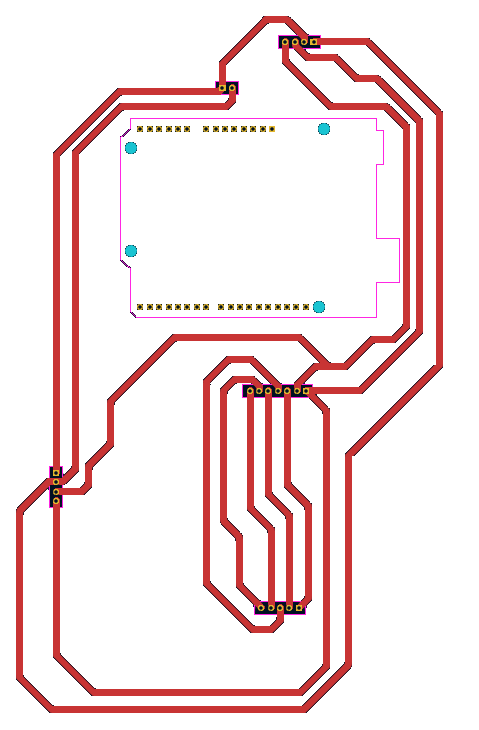
\includegraphics[width=0.6\textwidth]{images/layout.png}
    \caption{Rozkład ścieżek na płytce drukowanej}
    \label{fig:twoj_obrazek}
\end{figure}